% 公立はこだて未来大学 卒業論文 テンプレート ver1.50
% (c) Junichi Akita (akita@fun.ac.jp), 2003.10.31
% update by N.T.,  2004.11.10
%
\documentclass{funthesis}
%¥documentclass[english]{funthesis} % use [english] option for English style

\usepackage[dvips]{graphicx} % 図(EPS形式)を本文中で読み込む場合はこれを宣言
\usepackage{url}

% この部分に,タイトル・氏名などを書く.
% タイトルなどの定義の始まり
\jtitle{知識ベース型推薦を用いたフードツーリズム支援システムの構築}% 論文の和文タイトル
%
\etitle{Development of a Food Tourism Support System Using Knowledge-based Recommendation}% 論文の英文タイトル
%
\htitle{Development of a Food Tourism Support System Using Knowledge-based Recommendation}   % ヘッダー用の論文の短縮英文タイトル
%     必ず1行に収まるように英文タイトルを短縮する.
%
\jauthor{三好 良弥}     % 氏名(日本語)
\eauthor{Ryoya Miyoshi}   % 氏名(英語)
\jaffiliciation{情報アーキテクチャ学科} % 所属学科名(日本語)
\eaffiliciation{Department of Media Architecture} % 所属学科名(英語)
\studentnumber{1014127}   % 学籍番号
\jadvisor{奥野 拓}    % 正指導教員名(日本語)
%¥jcoadvisor{} % 副指導教員(日本語)がいる場合は
                        % コメントアウトし名前を書く
                        % 副指導教員がいない場合は,ここは削除しても可
\eadvisor{Taku Okuno}  % 正指導教員名(英語)
%¥ecoadvisor{}   % 副指導教員(英語)がいる場合は
                         % コメントアウトし名前を書く
                         % 副指導教員がいない場合は,ここは削除しても可
\jdate{平成30年01月29日}    % 論文提出日   (日本語)
\edate{January 29, 2018}     % 論文提出年月 (英語)
% タイトルなどの定義の終わり

\begin{document}

%--------------------------------------------------------------------
\maketitle       % タイトルページを作成

%--------------------------------------------------------------------
% 英文概要(250語程度)
\begin{eabstract}
In recent years, food tourism that a journey aimed at eating local cuisine is popular.
However, the criteria for regional dishes differ depending on the taste of tourists, it is difficult to find a local cuisine at a conventional gourmet site.
In order to solve this problem, I propose a local cuisine recommendation system considering the taste of tourists.
Extract information on restaurants and dishes using Web scraping.
We build a database using the extracted information and recommend a local cuisine to the taste of tourists.
As a recommendation method, by using Kowledge-based Recommender System that is effective when there is a specific condition that the user requires for the product.
\end{eabstract}

% 英文キーワード(5個程度をコンマ(,)で区切って羅列する)
\begin{ekeyword}
Food Tourism, Kowledge-based Recommender System, Preference Information
\end{ekeyword}

%--------------------------------------------------------------------
% 和文概要(300字程度)
\begin{jabstract}
近年,地域らしい料理を食べることを目的とした旅であるフードツーリズムが盛んである.
しかし,観光客の嗜好によって地域らしい料理の判断基準が異なるため,従来のグルメサイトでは地域らしい料理を探すことが困難である.
この問題を解決するために,観光客の嗜好を考慮した地域らしい料理推薦システムを提案する.
Webスクレイピングを用いてグルメサイトから飲食店及び料理の情報を抽出する.
その後,抽出した情報を用いてデータベースを構築し,観光客の嗜好にあった地域らしい料理の推薦を行う.
推薦手法として,「評価が高い商品」や「1000円以下の商品」などユーザが商品に求める具体的な条件がある場合に有効な知識ベース型推薦を用いることで,嗜好にあった料理の推薦を可能にする.
\end{jabstract}

% 和文キーワード(5個程度をコンマ(,)で区切って羅列する)
\begin{jkeyword}
フードツーリズム,知識ベース型推薦,嗜好情報
\end{jkeyword}

%--------------------------------------------------------------------
\tableofcontents % 目次を作成



%--------------------------------------------------------------------
% ¥includegraphics[width=??cm]{hoge.eps} % 図(EPS形式)を読み込む場合


%--------------------------------------------------------------------

\chapter{序論} 

\section{背景}
近年,ニューツーリズムの振興\cite{1}により,様々な物が観光資源となっている.その中でも,地域らしい料理が注目を浴びている.
地域らしい料理を食べることを目的とした旅のことをフードツーリズムと呼ぶ.
日本フードツーリズム協会\cite{2} は,フードツーリズムを,地域ならではの料理・食文化をその地域で楽しむための旅と定義している.

じゃらんが実施したアンケートの「宿泊旅行調査」の調査結果を図1.1に示す\cite{3}.
この調査によると,観光客が観光地を選んだ理由のひとつとして「地域らしい料理・特産品に興味があったから」と回答した人が2016年度は41.6\%であり,年々増加傾向であることがわかる.
このことから,観光客は地域らしい料理を旅行の際に重要視していることがわかる.

\begin{figure}[tbp]
  \begin{center}
    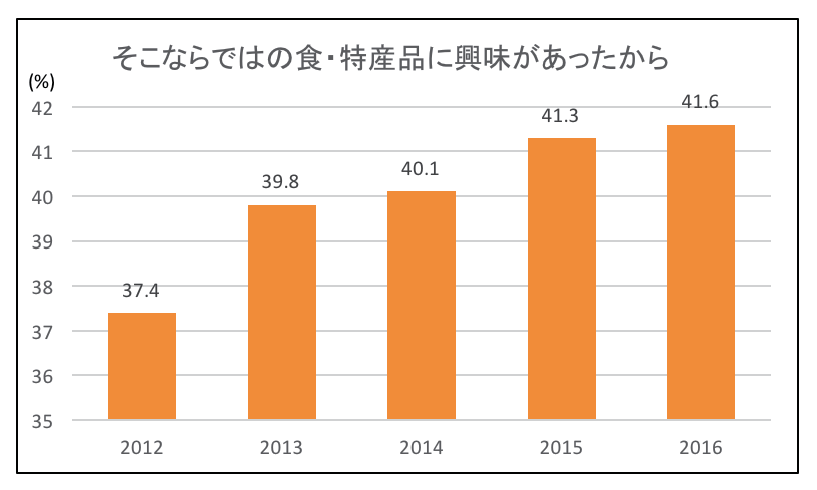
\includegraphics[clip,width=13cm]{jaran.eps}
    \caption{観光地を選ぶ理由}
  \end{center}
\end{figure}

観光客がフードツーリズムの重要な要素である地域らしい料理を探す方法の一つとしてグルメサイトを用いて検索する方法がある.
しかし,観光客によって地域らしい料理に求める条件が異なるため,観光客が期待する料理を探すことは容易ではないという問題がある.

\section{研究目的}  
本研究では観光客の嗜好や状況を考慮した地域らしい料理の推薦を行うことで観光客の満足度向上を目指す.
そこで,本研究では知識ベース型推薦を用いた地域らしい料理を推薦するシステムを提案する.

\section{本論文の構成}
本論文は全6章で構成されている.第1章では,本研究の背景および研究目的について述べた.
第2章では,関連研究について述べる.第3章では,推薦手法について述べる.第4章では,本研究で提案するフードツーリズム支援システムの構築について述べる.
第5章では,実験方法および実験の結果,結果から得られた考察について述べる.最後に第6章では,本研究のまとめと今後の展望を述べる.

%--------------------------------------------------------------------

\chapter{関連研究}
本章では,本研究と関連する研究を3つ述べる.
1つ目に地域特産の料理を検索するシステムについて述べる.
2つ目に旅行履歴を利用した観光地推薦の研究について述べる.
3つ目に旅行履歴を利用した観光地推薦の研究について述べる.

\section{地域特産の料理を検索するシステム}
地域のみで食べることのできる料理を簡単に探せるようにする研究として,地域特産の料理を検索するシステムの提案がある\cite{6}.
このシステムではグルメサイトをWebスクレイピングし,地域単位でメニューを抽出する.
その後,地域のメニューと首都圏のメニューを比較し地域のみで取り扱われている料理の検索を行えるようにしている.

この研究で用いている手法の場合,札幌におけるスープカレーなど,その地域で発祥したが,全国的に取り扱われている料理の場合,この手法では抽出ができない.
そのため,本研究では地域で発祥し,全国的に取り扱われている料理の抽出も可能にし,推薦を行えるようにする.

\section{旅行履歴を利用した観光地推薦の研究}
観光地の推薦をする研究として,協調ベース型推薦を用いた観光地推薦がある\cite{7}.
この研究では,システム利用者には今までの旅行履歴を入力してもらい,入力した旅行履歴と観光地の特徴を用いて,
旅行計画者が入力した嗜好にあった新たな観光地の推薦を行っている.

この研究で用いている手法の場合,ユーザに旅行経験があるということを前提としている.しかし,旅行経験がないというユーザの場合,
嗜好情報の取得が難しく,適切な観光地を推薦することができない問題がある.

\section{食材の利用履歴を利用したレシピ推薦の研究}
レシピの推薦をする研究として,ナイーブベイズ分類器を用いた,
栄養素のバランスと嗜好を考慮した食事レシピの推薦を行うシステムの提案がある\cite{8}.
この研究では,食材から得られる栄養素と過去に調理したレシピに使われている調味料を用いて,
ユーザの味の嗜好に合致し,不足している栄養素を摂取できるレシピの推薦を行う.

料理を推薦する際,味という嗜好はとても重要な要素と考えられる.しかし,各店舗によって料理の味付け方法は異なり,
実際に食べてみないと分からないため,味付けの分類が難しい問題がある.

%--------------------------------------------------------------------

\chapter{推薦手法}
本章では,嗜好を用いて情報を推薦する手法について述べた後,本研究で用いる手法について述べる.

\section{嗜好を用いた情報推薦手法}
情報推薦に用いられる代表的な手法は,協調ベース型推薦,内容ベース型推薦,知識ベース型推薦がある\cite{4}.
それぞれの手法について以下で述べる.

\subsection{協調ベース型推薦}
協調ベース型推薦とは,類似したユーザの嗜好や過去の行動からユーザが好むであろうアイテムを推薦する手法である.
この手法はamazon\cite{5}のおすすめなどショッピングサイトの商品推薦で用いられている.

以下に,協調ベース型推薦を用いて商品を推薦する例を示す.
表2.1は各ユーザの商品への嗜好を示している.この例ではユーザDに商品Dを推薦するのが適切かを判断する.
各ユーザの嗜好を比較すると,ユーザAとユーザDの嗜好が類似していることがわかる.
このことから,ユーザAが好きである商品DはユーザDも好むと予測できるため,ユーザDに商品Dを推薦することが適切だと判断するものである.

\begin{table}[htb]
  \begin{center}
  \scriptsize
    \caption{協調ベース型推薦を用いた商品を推薦する例}
    \normalsize
   \begin{tabular}{p{2.5cm}||p{2.5cm}|p{2.5cm}|p{2.5cm}|p{2.5cm}}
    \hline
ユーザ & 商品A & 商品B & 商品C & 商品D \\ \hline\hline
      ユーザA & 好き & 好き & 嫌い & 好き \\ \hline
      ユーザB & 好き & 嫌い & 好き & 好き \\ \hline
      ユーザC & 嫌い & 好き & 嫌い & 好き \\ \hline
      ユーザD & 好き & 好き & 嫌い & ? \\ \hline
  \end{tabular}
  \end{center}
\end{table}

\subsection{内容ベース型推薦}
内容ベース型推薦とは,ユーザの好むアイテムと類似したアイテムを推薦する手法である.

以下に,内容ベース型推薦を用いて料理を推薦する例を示す.
表2.2はユーザの好む料理の特徴と,各料理の特徴を示している.
この例ではユーザに新たな料理を推薦する際,どの料理を推薦するのが適切かを判断する.
ユーザと各料理の特徴を比較すると,料理Bの特徴とユーザの好む特徴が類似していることがわかる.
このことから,ユーザは料理Bも好むと予測できるため,料理Bを推薦することが適切だと判断するものである.

\begin{table}[htb]
  \begin{center}
  \scriptsize
    \caption{内容ベース型推薦を用いた料理を推薦する例}
    \normalsize
   \begin{tabular}{p{2.5cm}|p{2.5cm}||p{2.5cm}|p{2.5cm}|p{2.5cm}}
    \hline
    & ユーザ & 料理A & 料理B & 料理C  \\ \hline\hline
      ジャンル & 洋食 & 和食 & 洋食 & 和食 \\ \hline
      価格 & 1000円 & 800円 & 2000円 & 1000円 \\ \hline
      味 & 甘い & 辛い & 甘い & しょっぱい \\ \hline
  \end{tabular}
  \end{center}
\end{table}

\subsection{知識ベース型推薦}
知識ベース型推薦とは,ユーザに「予算は2000円,料理のジャンルは洋食が良い」など具体的な好みを示してもらい,示された好みを満たす商品に絞り込み,
ユーザへの効用が高くなるようにソートを行い,上位の商品を提示する手法である.
ユーザにあったソートを行うため,一般的な推薦システムで行われている人気順などのソートと比べ,推薦された商品に対するユーザの満足度が高くなるという特徴がある.

以下に,知識ベース型推薦を用いてカメラを推薦する例を示す.
表2.3は各カメラの特徴を示している.
この例ではユーザがカメラを選ぶ際に具体的な好みがある場合,どのカメラを推薦するのが適切かを判断する.
ユーザから「予算は30000円,5倍以上のズームができる,機能重視」という好みがあった場合,この条件を満たすカメラBとカメラDを推薦候補とする.
その後,推薦候補の中で「機能重視」という情報からソートを行い,カメラBを推薦リストの上位にすることが適切だと判断するものである.

\begin{table}[htb]
  \begin{center}
  \scriptsize
    \caption{知識ベース型推薦を用いたカメラを推薦する例}
    \normalsize
   \begin{tabular}{p{3.3cm}||p{3.3cm}|p{3.3cm}|p{3.3cm}}
    \hline
カメラ & 価格 & ズーム & 液晶サイズ \\ \hline\hline
      カメラA & 40000円 & 10倍 & 3インチ \\ \hline
      カメラB & 30000円 & 10倍 & 3インチ \\ \hline
      カメラC & 15000円 & 4倍 & 2.5インチ \\ \hline
      カメラD & 20000円 & 5倍 & 2.7インチ \\ \hline
  \end{tabular}
  \end{center}
\end{table}

\section{本研究で用いる手法}
本研究では,知識ベース型推薦を用いる.
その理由として,協調ベース型推薦を対象とする問題に用いた場合,料理の「価格」や「カテゴリ」などの属性を考慮した推薦を行えないという問題がある.
また,内容ベース型推薦を用いた場合,「地域らしい料理を食べる」という観光の際にのみ行われる稀な事象は嗜好情報を得ることが難しいという問題がある.
ユーザは料理や店舗の属性を考慮して料理を選択するため,ユーザの選択した属性と置かれた状況を考慮した推薦を行える知識ベース型推薦を用いて推薦を行う.

%--------------------------------------------------------------------
\chapter{提案手法}

\section{推薦アルゴリズム}
本研究で用いた知識ベース型推薦のアルゴリズムを図1に示す.以下に顧客要求と製品制約,効用にもとづくソートについて記述する.

\begin{figure}[!b]
  \begin{center}
    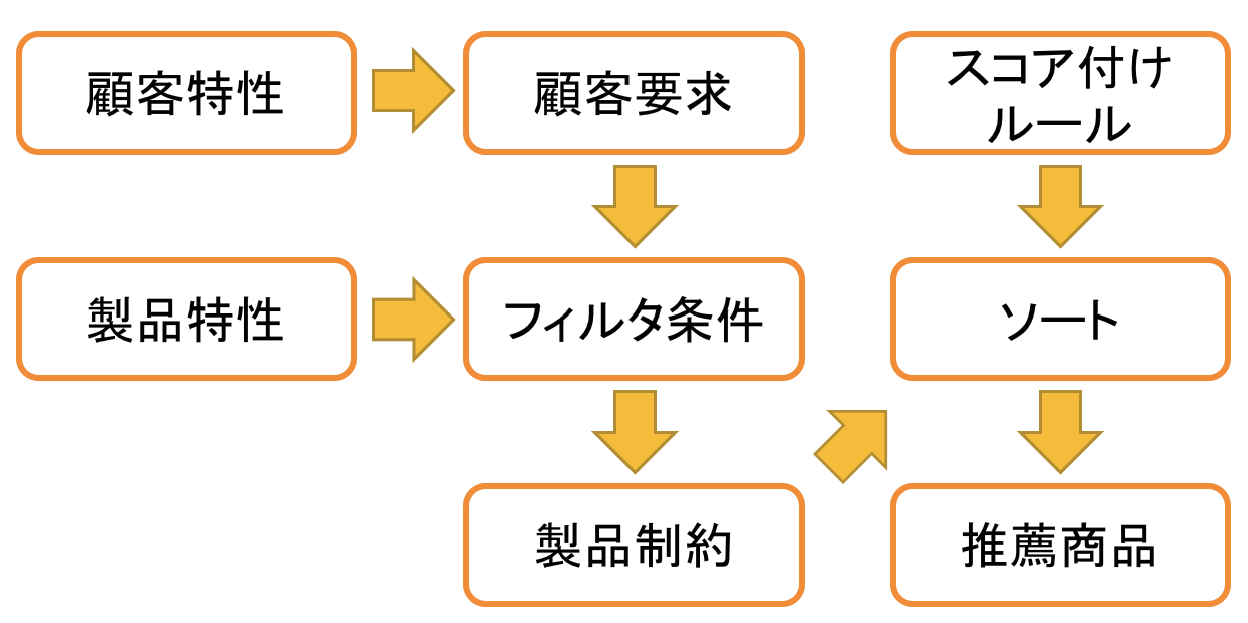
\includegraphics[clip,width=13cm]{model.eps}
    \caption{知識ベース型推薦のアルゴリズム}
  \end{center}
\end{figure}

\subsection{顧客要求}
知識ベース型推薦では,顧客特性をもとに顧客要求を設定する.
顧客特性とは,ユーザが商品を選ぶ際に使用する項目の集合である.本研究では顧客特性に,予算,ジャンルを使用する.
顧客要求とは,ユーザがどのような顧客特性を持っているかをまとめた集合である.本研究での顧客要求の例として「予算は1000円,ジャンルは洋食の料理が食べたい」が挙げられる.

\subsection{製品制約}
知識ベース型推薦では,顧客要求と製品特性をもとにフィルタ条件を用いて,ユーザが満たして欲しい条件を設定する.
本研究において製品特性とは,料理及び店舗が持つすべての属性である.本研究で定義した製品特性の例を表1,2に示す.
フィルタ条件とは,顧客要求と製品特性との関係を定義したものである.例えば,顧客要求として「予算が1000円」と入力された場合,「価格」が1000円以下の料理に絞り込む.
以上をもとに製品制約に使用するSQLを生成した.

\begin{table}[htb]
  \begin{center}
  \scriptsize
    \caption{製品特性の例(料理)}
    \normalsize
    \begin{tabular}{p{6cm}|p{6cm}}
    \hline
属性 & 値 \\ \hline\hline
      料理id & 149\\ \hline
      料理名 & 塩ラーメン \\ \hline
      価格(円) & 580 \\ \hline  \end{tabular}
  \end{center}
  \end{table}
  
\begin{table}[htb]
  \begin{center}
  \scriptsize
    \caption{製品特性の例(店舗)}
    \normalsize
   \begin{tabular}{p{6cm}|p{6cm}}
    \hline
属性 & 値 \\ \hline\hline
      店舗id & 6\\ \hline
      店名 & 星龍軒 \\ \hline
      住所 &  北海道函館市若松町7-3\\ \hline
      オープン年(年)& 1951 \\ \hline
      ジャンル & ラーメン、餃子、中華料理 \\ \hline
      緯度 & 41.771268 \\ \hline
      経度 & 140.7264993 \\ \hline
  \end{tabular}
  \end{center}
\end{table}

\subsection{効用にもとづくソート}
知識ベース型推薦では,効用に基づくソートを行う.
本研究では,「地域発祥の料理」,「古くからある店舗」,「地域でしか食べられない料理」,「人気のある料理」の4項目の観点でユーザの効用を求め,ソートを行う.
効用は式(1)で求めることができる.

\begin{equation}
効用(p)=\sum_{j=1}^{n} 関心度(j)×貢献度(p,j) 
\end{equation}

{\it p}は料理,{\it j}は観点を表す.関心度とはある観点においてどれほど商品に関心があるのかを表した度合いである.
本研究では関心度をユーザに入力してもらう.貢献度とは商品がある観点にどれだけ貢献しているかを表した度合いである.
本研究ではスコア付けルールを用いて貢献度を設定する.スコア付けルールとは料理および店舗の属性をもとに本研究で定義した観点を数値化するものである.
以下で,各観点の貢献度の求め方を示す.

\subsubsection{地域発祥の料理}

\subsubsection{古くからある店舗}

\subsubsection{地域でしか食べられない料理}

\subsubsection{人気のある料理}

\section{使用するデータの収集}
本研究では,函館市で取り扱われている「食べログ」\cite{4},「ぐるなび」\cite{5}からWebスクレイピングにより函館市の料理および飲食店の情報を収集した.
収集した情報は表1,2の各属性と店舗の口コミである.収集した情報で店舗名が一致するものを同一店舗とみなし情報を統合させ,推薦の際に使用するデータベースを構築した.
収集した情報は,飲食店の情報が2,206件,料理の情報が9,866件,口コミの情報が14,974件である.
他の属性として,料理に使われている材料の情報などを利用することを考えていたが,本研究では収集することができなかった.

\section{システムの実装}
本研究では5.1,5.2節をもとにWeb上で利用できるフードツーリズム支援システムを構築した.構築したシステム画面を図2に示す.
ユーザの要求を入力する手段として,セレクトボックス,テキストボックス,スライダを用いる.
推薦結果は,ユーザへの効用が高い上位8件を表示する.また,推薦された料理を取り扱っている店舗の場所がわかるように,マップにマーカーを設置し店舗の位置を表示する.

\begin{figure}[!p]
  \begin{center}
    \includegraphics[clip,width=13cm]{test1.eps}
    \caption{システム画面(初期画面)}
  \end{center}
\end{figure}

\newpage

\begin{figure}[!p]
  \begin{center}
    \includegraphics[clip,width=13cm]{test.eps}
    \caption{システム画面(入力後画面)}
  \end{center}
\end{figure}

%--------------------------------------------------------------------
\chapter{実験}

%--------------------------------------------------------------------
\chapter{結論}

\section{まとめ}

\section{今後の展望}

\chapter *{謝辞}
本研究にあたりご指導いただいた指導教員の奥野拓准教授に深くお礼申し上げます.
また,様々な助言をしていただいた奥野研究室の皆様,本研究に関わった方々にも深くお礼申し上げます.



%--------------------------------------------------------------------
% 参考文献
\begin{thebibliography}{7}
\end{thebibliography}

% 表目次の表示
\listoftables

% 図目次の表示
\listoffigures

\end{document}
